\section{Project Plan}

\subsection{Project Estimate}
%\paragraph{ESTIMATE DESC}
\subsubsection{Reconciled Estimates}
\subsubsection{\textbf{Cost Estimate}}
Cost of project\\
C=N*Cp\\
C=3*8000\\
C=24,000\\
The Cost of the project is approximately up to 24000/-
\subsubsection{\textbf{Time Estimates}}
\textbf{Line of Code (LoC):}
\begin{flushleft}
	Estimating LOC for this project is difficult at estimation stages this project is of innovative
	type project. Average estimation of this project is 10000 to 12000 line of code.
\end{flushleft}
\textbf{LOC based Estimation:}\\ \\
\textbf{Efforts in Person in months}\\ \\
\(E=3.2*(KLOC)^1 .05 \) \\
\(E=3.2*9.0^1 .05 to 11.0 *4.2^1 .05\)\\
\begin{flushleft}
	\begin{Table}
		\begin{center}
			\def\arraystretch{1.5}
			\begin{tabular}{ |p{4.2cm}|p{4.8cm}| }
				\hline
				\textbf{Function} & \textbf{Estimated KLOC} \\
				\hline
				GUI design & 1.1-1.3\\
				\hline
				Logical code & 1.5-2.0\\
				\hline
				Location Based code & 1.1-1.3\\
				\hline
				Directory matching code & 1.0-1.3\\
				\hline
				Business logic & 2.2-2.5\\
				\hline
				Testing & 1.1-1.2\\
				\hline
				Re-correct Code & 1.0-1.2 \\
				\hline
				Total & 9.0-10.11\\
				\hline
			\end{tabular}
			\caption{LOC Based estimation }
			\label{tab:LOC Based estimation}
		\end{center}
	\end{table}\\\\
	
\end{flushleft}
\\\\ \newline
\subsubsection{\textbf{Man Month Utilization:}}
Estimation of the man month is divide into following sub activities:\\
1-Technical training of the team member: This will take nearly 1 months. This will include Advance java, mysql, serialization etc.\\
2-Research: Being an innovative project research for the project is an important part currently it seems to have 1 to 1.5 months

\subsubsection{Project Resources}
         \begin{itemize}
	\item \textbf{Hardware Resources Required:}
	
	\begin{enumerate}
		\item Processor: Intel i3
		\item Hard Disk: Minimum 100GB
		\item RAM: 4GB
	\end{enumerate}
\end{itemize}

\begin{itemize}
	\item \textbf{Software Resources Required:}
	
	\begin{enumerate}
		\item Platform: Windows7 and above.
		\item Backend: Mysql 5.5.0
		\item Front End: JAVA.
	\end{enumerate}
\end{itemize} 

\subsection{Risk Management}
\begin{itemize}
	\item	In appropriate dataset -To overcome this risk we are trying to use well organized and complete dataset. 
	\item	Security- To overcome and  improving  security we use multilevel security like access permissions of user.
\end{itemize}
When solving problems we have to decide the difficulty level of our problem. There are three types of classes provided for that. These are as follows:
\begin{itemize}
	\begin{enumerator}
		\item P class
		\item NP-Hard Class
		\item NP Complete Class
	\end{enumerator}
\end{itemize}
\textbf{P Class:-}\\
\justify\hspace{2cm}In computational complexity theory, P, also known as PTIME or DTIME(nO(1)), is a fundamental complexity class. It contains all decision problems that can be solved by a deterministic Turing machine using a polynomial amount of computation time, or polynomial time.P class problems are deterministic problems i.e. P class problems can be solve by deterministic Turing Machine.\\
\textbf{Np Class:-}\\
\justify\hspace{2cm}In computational complexity theory Equivalently, the formal definition of NP is the set of decision problems solvable in polynomial time by a theoretical non-deterministic Turing machine. This second definition is the basis for the abbreviation NP, which stands for "nondeterministic, polynomial time." However, the verifier-based definition tends to be more intuitive and practical in common applications compared to the formal machine definition. The two definitions are equivalent because the algorithm for the machine definition consists of two phases, the first of which consists of a guess about the solution, which is generated in a non-deterministic way, while the second phase consists of a deterministic algorithm that verifies or rejects the guess as a valid solution to the problem.\\

\begin{flushleft}
	\textbf{3. NP Hard Class:-}
	
	\begin{itemize}
		\item NP-hardness stands for Non-deterministic polynomial-time hard.
		\item Informally, "at least as hard as the hardest problems in NP" are called as NP hard class problem.
	\end{itemize}
\end{flushleft}


\subsubsection{Risk Identification}
For risks identification, review of scope document, requirements specifications and schedule is done. 
\begin{enumerate}
	\item Have top software and customer managers formally committed to support the project?\\
	Ans: All the required software’s are freely available and hence development will be possible.
	\item Are end-users enthusiastically committed to the project and the system/product to be built?\\
	ans: The end user will be developers itself.
	\item Are requirements fully understood by the software engineering team and its customers?\\
	Ans: Yes. All the requirements are fully understood by our team.
	\item Have customers been involved fully in the definition of requirements?\\
	Ans: This is academic level project. So that whatever requirement be specify it should be by our team members and our guide.
	\item Do end-users have realistic expectations?\\
	Ans: Yes.
	\item Does the software engineering team have the right mix of skills?\\
	Ans: Yes, we have.
	\item Are project requirements stable?\\
	Ans: All the basic requirements for this project are stable, from though some being variable but can be fulfilled.
	\item Is the number of people on the project team adequate to do the job?\\
	Ans: Yes.
	\item Do all customer/user constituencies agree on the importance of the project and on the requirements for the system/product to be built?\\
	Ans: Yes.
\end{enumerate}
\newpage
\subsubsection{Risk Analysis}
The risks for the Project can be analyzed within the constraints of time and quality.

\begin{figure}[h!]
	\centering
	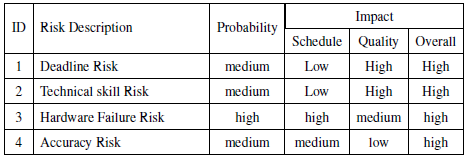
\includegraphics[width=.95\linewidth]{./r1}
		\caption{Risk Table}
	\label{fig:Risk Table}	
	\end{figure}


\begin{table}[htbp]
	\begin{center}
		%\def\arraystretch{1.5}
		\def\arraystretch{1.5}
		\begin{tabular}{| c | c | c |}
			\hline
			Probability & Value &	Description \\ \hline
			High &	Probability of occurrence is &  $ > 75 \% $ \\ \hline
			Medium &	Probability of occurrence is  & $26-75 \% $ \\ \hline
			Low	& Probability of occurrence is & $ < 25 \% $ \\ \hline
		\end{tabular}
	\end{center}
	\caption{Risk Probability definitions}
	\label{tab:riskdef}
\end{table}
\newpage
\subsection{Overview of Risk Mitigation ,Monitoring,Management}
\begin{figure}[h!]
	\centering
	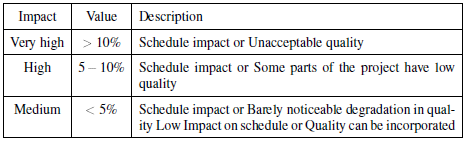
\includegraphics[width=.95\linewidth]{./r2}
		\caption{Risk Impact definitions}
		\label{fig:Risk Impact definitions}	
	\end{figure}

\begin{figure}[h!]
	\centering
	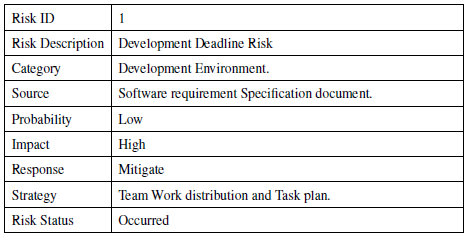
\includegraphics[width=.95\linewidth]{./r3}
		\caption{Risk Impact definitions}
		\label{fig:Risk Impact definitions}	
		
	\end{figure}
\begin{figure}[h!]
	\centering
	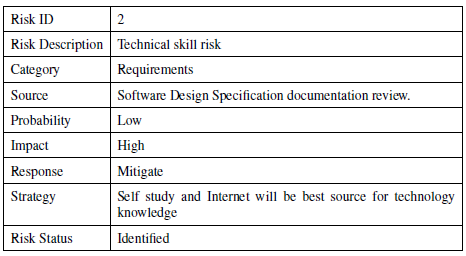
\includegraphics[width=.95\linewidth]{./r4}	
	\end{figure}
\newpage
\begin{figure}[h!]
	\centering
	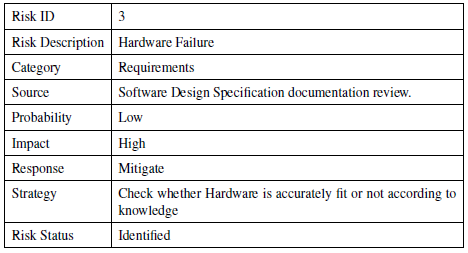
\includegraphics[width=.95\linewidth]{./r5}
			
		
	\end{figure}
\begin{figure}[h!]
	\centering
	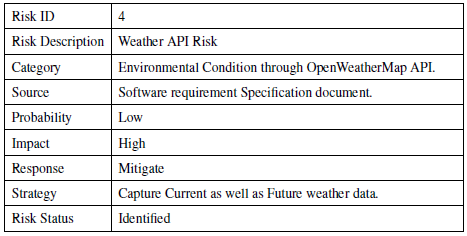
\includegraphics[width=.95\linewidth]{./r6}		
	\end{figure}
%\begin{table}[hp!]
%\caption {Risk Analysis}
%\begin{tabular}{|p{4cm}|p{3cm}|p{7cm}|}
%\hline  Risk & Probability & Mitigation \\ 
%\hline  It takes longer than proposed to learn the new technologies 	& Low &  
%\begin{enumerate}
%\item	Advanced concepts are learnt on need-to-know basis and basic features are prioritized which are required for the implementation
%\item	Rescheduling of the project plan to accommodate any delay
%\end{enumerate}\\ 
%\hline Some technical problem arise during implementation & Low & Help from developer community from various blogs and forums can be taken \\ 
%\hline
%\end{tabular} 
%\end{table}

\subsection{Project Schedule}

\subsubsection{Project Task Set}
Major Tasks in the Project stages are:\\
\begin{itemize}
	\item Task 1.1: Checking Feasibility of product
	\item Task 1.2: Scope of Product
	\item Task 1.3: Product Planing
	\item Task 1.4: Technical Risk
	\item Task 1.5: Proof of product
	\item Task 1.6: Implementation
	\item Task 1.7: Costumer Feedback
\end{itemize}
\newpage
\subsection{Task network}  
Project tasks and their dependencies are noted in this diagrammatic form.
\begin{center}
	\begin{figure}[!h]
		\centering
		\fbox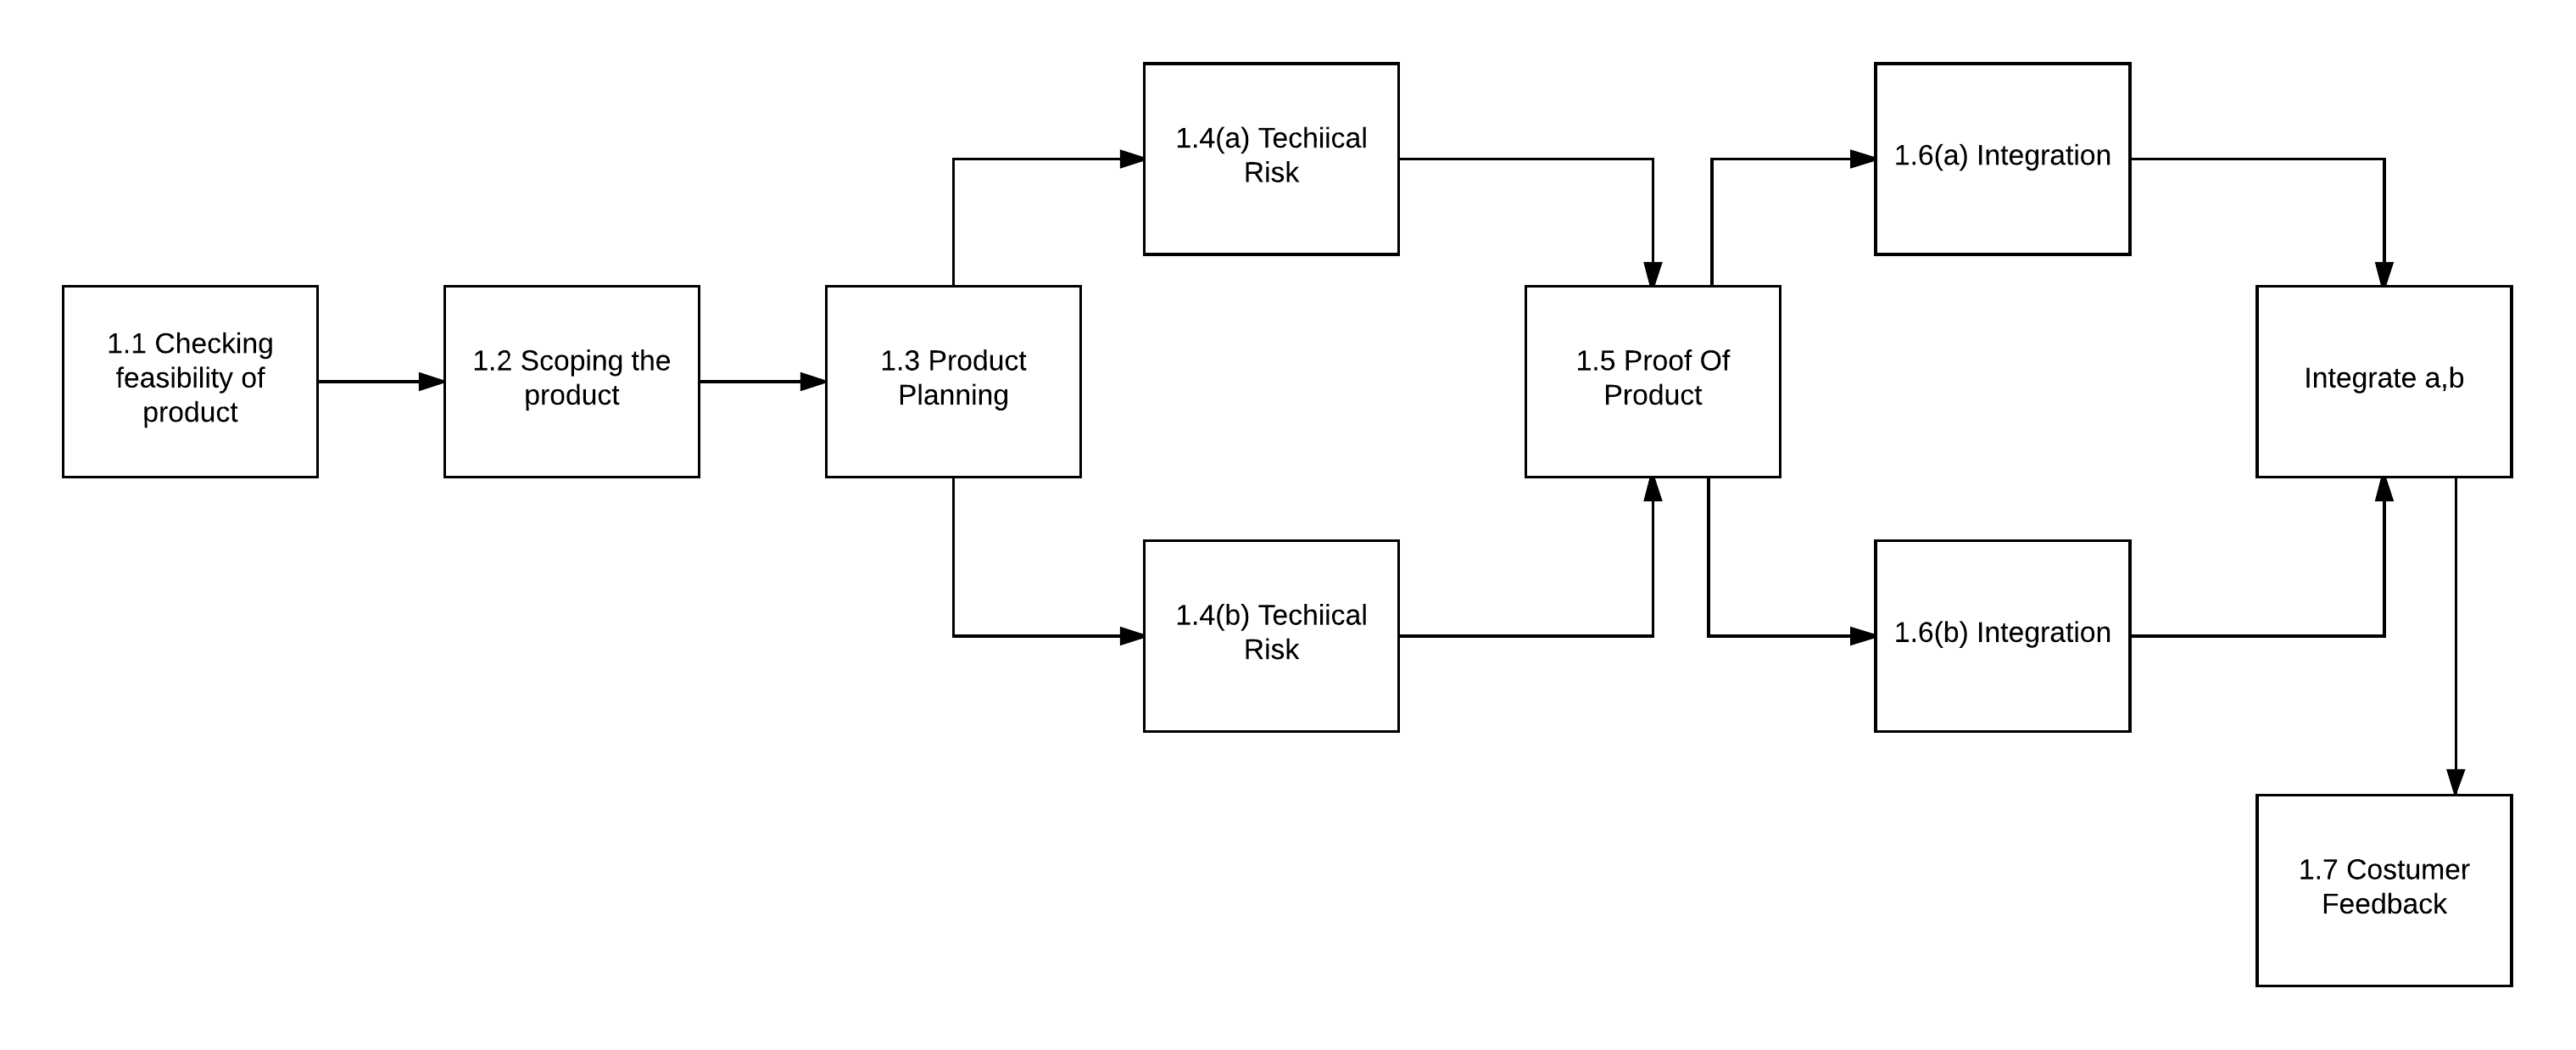
\includegraphics[height=7.5cm,width=16cm]{./tasknw}}
		\caption{Task Network}
		\label{fig:Task Network}
	\end{figure}
\end{center}
\subsubsection{Time line Chart}

\begin{figure}[h]
\centering
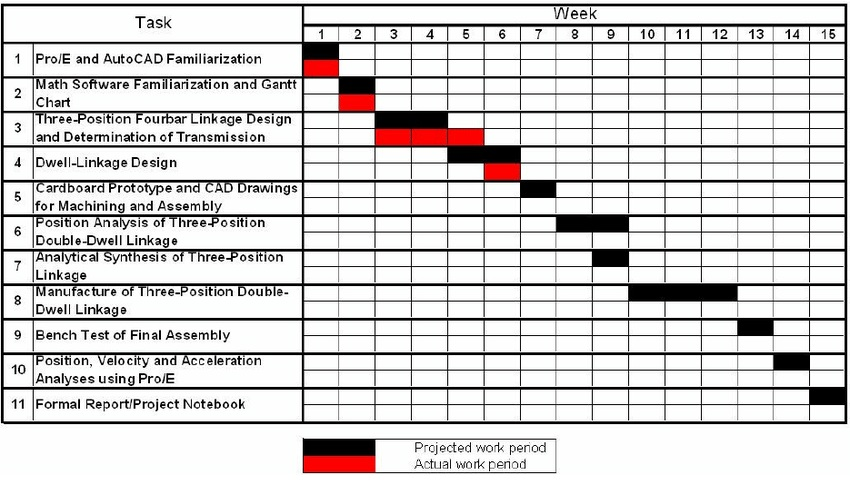
\includegraphics[width = \textwidth]{./sem1plan}
\caption{Timeline of Literature review}
\end{figure}

\begin{figure}[!h]
\centering
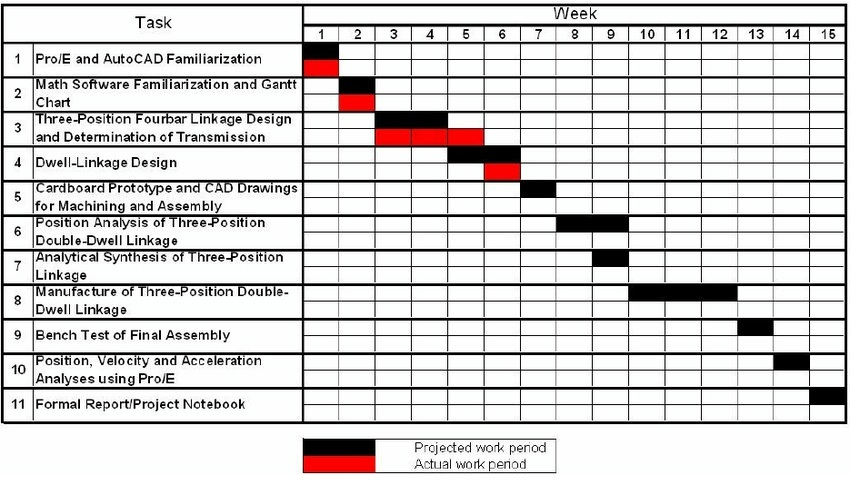
\includegraphics[width = \textwidth]{./sem2plan}
\caption{Timeline of Project Stage 1}
\end{figure}
\newpage
\subsection{Team Organization}
\subsubsection{Team Structure}
The team structure for the project is identified. Roles are defined. Our team
have three members. We select this topic after discussing with each other. All the
members performing all the task whatever tasks are assign to the members.
Team Member Details:-\\
Sanket sopan  shirse 
Shubham  Ajit asabe  
Rohan mandar salvi  
Vipul bhausaheb ahire 
\subsubsection{Management reporting and communication}
\begin{Table}
	\def\arraystretch{1.5}
	\begin{tabular}{ |p{1.2cm}|p{2.8cm}|p{9cm}| }
		\hline
		\textbf{SR.NO} & \textbf{Reporting Date} & \textbf{Project Activity}\\
		\hline
		1 & 22 June 2020 & Decide project group member\\
		\hline
		2 &29 June 2020 & Submitted 3 Project Topic with IEEE Paper\\
		\hline
		3 &13 Jul 2020 & Discuss 5 point analysis of selected IEEE Paper\\
		\hline
		4 &20 Jul 2020 & 3 Topics are presented and 1 topic selected\\
		\hline
		5 &27 Jul 2020 & Created and Submitted synopsis of a selected project\\
		\hline
		6 &3 Aug 2020 & Literature Survey and info gathering of a selected project\\
		\hline
		7 &10 Aug 2020 & 30 percent project completion and presentation\\
		\hline
		8 &31 Aug 2020 & Draw UML diagram of a project\\
		\hline
		9 &31 Aug 2020 & 50 percent project completion and presentation\\
		\hline
		10 &7 Feb 2020 & 100 percent project completion and presentation\\
		\hline
		11 &3 March 2021 &Show the paper published\\
		\hline
		12 &23 March 2021 & Show the final report\\
		\hline
		13 &6 April 2021 & Show the final PPT\\
		\hline
		14 &9 May 2021 & Term 1st Project overview\\
		\hline
	\end{tabular}
	\caption{Team work distribution }
	\label{tab:Team work distribution}
\end{table}


